%!TEX root = ./ERL Industrial Robots.tex


%--------------------------------------------------------------------
%--------------------------------------------------------------------
\subsection{Control Functionality}
\label{ssec:Control}
%--------------------------------------------------------------------
\subsubsection{Functionality Description}
\label{sssec:ControlDescription}
This functionality benchmark assesses the robot's capability to control the manipulator's (and the mobile platform's) motion in a continuous manner. This functionality is essential for precise placement of objects (see TBM2 in Section \ref{ssec:TaskPlateDrilling}) or following a given line in common industrial applications like welding or gluing.
A marker set is attached to the robot's manipulator. With the tip of this marker set, the robot has to follow a given path in Cartesian space. The external ground truth system measures the deviation between the given path and the path executed by the robot using this marker.
Only for visualization purposes, the path is displayed on the table (see Figures \ref{fig:FBM3_line_example} and \ref{fig:FBM3_sine_example}).


%--------------------------------------------------------------------
\subsubsection{Feature Variation}
\label{sssec:ControlVariation}

The path is a segment of either a straight line or a sine function.
In future competitions the path can be given as a trajectory including velocities and accelerations.
The path can be limited to the workspace for a manipulator or of a size that forces the mobile platform to move as well (future competitions).

%--------------------------------------------------------------------
\subsubsection{Input Provided}
\label{sssec:ControlInput}

\paragraph{Marker set}
An image of the marker set is depicted in Figure~\ref{fig:MarkerSetEndEffector}. The rod of this marker set is attached either directly to the end-effector or to the tool on the robot's manipulator. The tip of the marker set is defined as the center of the spherical cap nut at the end of the rod. This tip is indicated by the coordinate frame in Figure \ref{fig:MarkerSetEndEffector}. Note that in this FBM only the origin of the coordinate frame is important, while the orientation is irrelevant!
\begin{figure}[!htbp]
	\begin{center}
		\subfigure[]{
			\includegraphics[width=0.45\textwidth]{fig/marker_set/marker_set_with_frame}
			\label{fig:MarkerSetEndEffectorWithFrame}
		}
		\subfigure[]{
			\includegraphics[width=0.45\textwidth]{fig/marker_set/marker_set_side}
			\label{fig:MarkerSetEndEffectorSide}
		}
		\caption{The marker set used in FBM3. The rod is marked by the yellow brace. The tip of the marker set is marked by the origin of the coordinate frame (the orientation of the coordinate frame is irrelevant here).}
		\label{fig:MarkerSetEndEffector}
	\end{center}
\end{figure}

\paragraph{Path specification}
The path to be executed by the robot is specified by:
\begin{itemize}
\item a mathematical description of a line in 2D space (see Figure~\ref{fig:FBM3_line_example} for an example):
    \begin{displaymath}
    f(x) = m \cdot x
    \end{displaymath}
    where
    \begin{itemize}
    \item $x$ is a distance in metres [$m$] along the x-axis of the robot-selected coordinate system
    \item $f(x)$ is a distance specified in metres [$m$] along the y-axis of the robot-selected coordinate system
    \item $m$ is the slope specified as a dimensionless scalar
    \end{itemize}
\item a mathematical description of a sine in 2D space (see Figure~\ref{fig:FBM3_sine_example} for an example):
    \begin{displaymath}
    f(x) = a \cdot \sin(c \cdot x)
    \end{displaymath}
    where
    \begin{itemize}
    \item $x$ is a distance in metres [$m$] along the x-axis of the robot-selected coordinate system
    \item $f(x)$ is a distance specified in metres [$m$] along the y-axis of the robot-selected coordinate system
    \item $a$ is the amplitude specified in metres [$m$]
    \item $c$ is a conversion from a distance to an angle specified in radians per metre [$\frac{rad}{m}$].
    \end{itemize}
\item distance between the calibration point and starting point specified in metres [$m$].
\item start of the path, specified in the domain of the mathematical description.
\item end of the path, specified in the domain of the mathematical description.
\item the concrete selection of the parameters for each benchmark will be announced before the competition.
\end{itemize}
\noindent
To exemplify the definition of start and end of the path assume a sine with $a = 0.1\;m$ and $c = 12.5\cdot\pi\;\frac{rad}{m}$. Let the start of the path be given as $start = 0\;m$ and the end of the path be given as $end = 0.2\;m$. Then the start point is $f(start = 0\;m) = 0\;m$ and the end point is $f(end = 0.2\;m) = 0.1 \;m$.

\begin{figure}[!htbp]
	\begin{center}
		\frame{\includegraphics[scale=0.5,angle=0]{fig/FBM/atwork/fbm3/fbm3_line_example.pdf}}
		\caption{Example of a path on a straight line.}
		\label{fig:FBM3_line_example}
	\end{center}
\end{figure}

\begin{figure}[!htbp]
	\begin{center}
		\frame{\includegraphics[scale=0.4,angle=0]{fig/FBM/atwork/fbm3/fbm3_sine_example.pdf}}
		\caption{Example of a path on a sine.}
		\label{fig:FBM3_sine_example}
	\end{center}
\end{figure}

\begin{figure}[!htbp]
	\begin{center}
		\frame{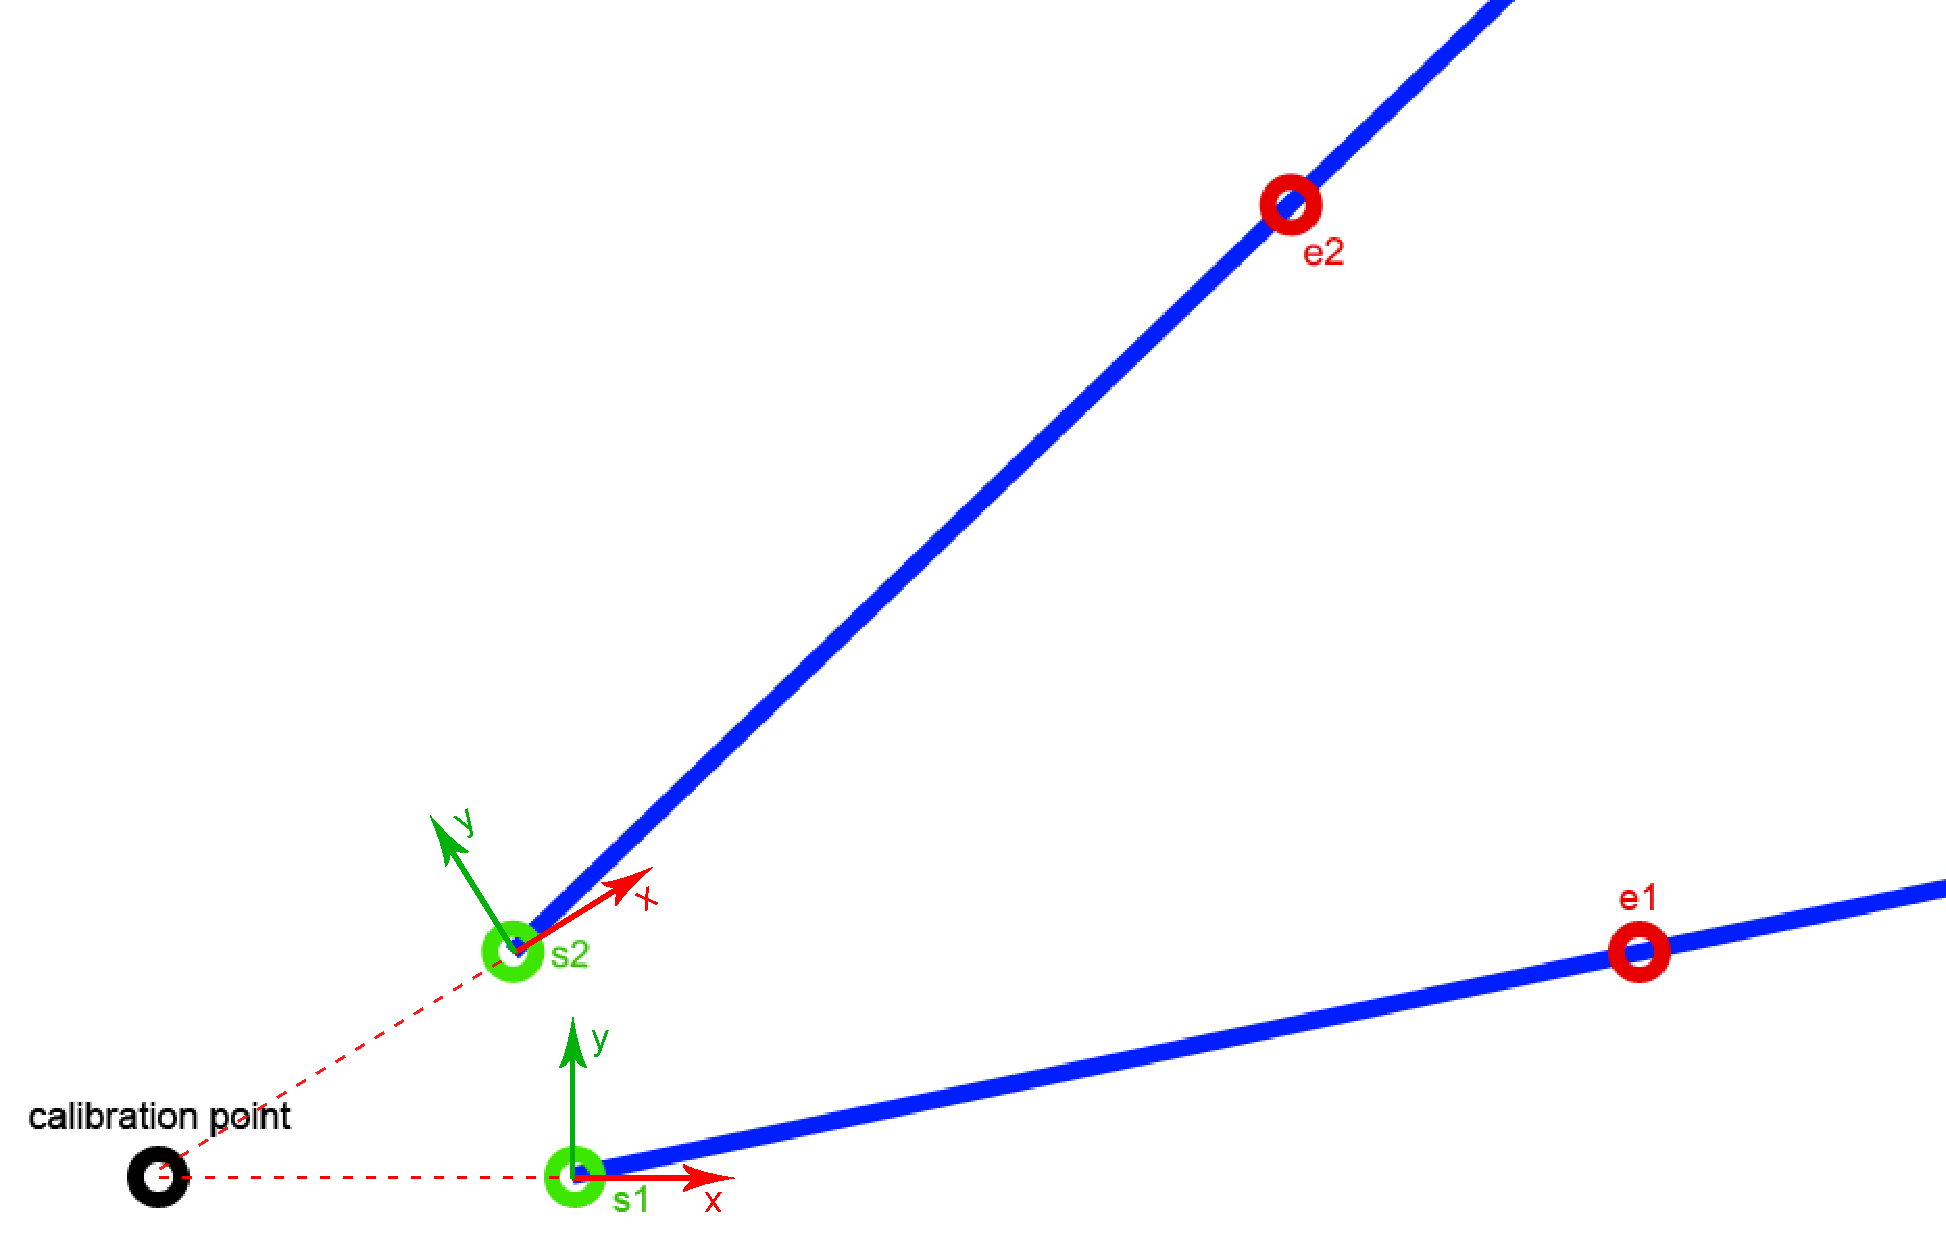
\includegraphics[scale=0.4,angle=0]{fig/FBM/atwork/fbm3/fbm3_rotation_example.pdf}}
		\caption{Example of two different starting points, $s1$ and $s2$. Note that the orientation of the path depends on the starting point.}
		\label{fig:FBM3_rotation_example}
	\end{center}
\end{figure}

%--------------------------------------------------------------------
\subsubsection{Expected Robot Behaviour or Output}
\label{sssec:ControlOutput}

The robot is placed in front of the test area (a planar surface). The robot is required to execute the provided path in a plane above the test area that is parallel to the ground, where the height above the ground is selected by the robot. Because the robot is free to select the reference frame w.r.t. which the path is executed, it must synchronize its internal reference frame with the benchmarking system's reference frame. This is achieved by a two-step calibration procedure as described below.

Each benchmark run consists of three different phases, namely \emph{calibration}, \emph{preparation} and \emph{execution}. In the calibration phase the robot moves the tip of the marker set to an arbitrary point on top of the test area which will be used as the \emph{calibration point}. Afterwards, in the preparation phase, the robot must move the tip of the marker set by the predefined \emph{calibration distance} (see Figure \ref{fig:FBM3_line_example} and Figure \ref{fig:FBM3_sine_example}) in a self-selected direction. The position reached after that motion is defined as the \emph{starting point} of the path. Finally, in the execution phase, the robot follows the path until the end point is reached or the time runs out. After each phase, the robot notifies the CFH that it has completed the phase.

The robot-selected coordinate system is derived based on the calibration procedure in the following way:
\begin{enumerate}
	\item The \emph{x-axis} is defined as the vector from the calibration point to the starting point.
	\item The \emph{z-axis} points upwards from the test area.
	\item The \emph{y-axis} complements the right-handed coordinate system.
\end{enumerate}
Figure~\ref{fig:FBM3_rotation_example} depicts two examples of such robot-selected coordinate systems.

Notice: this task is NOT executed with a feedback from any vision sensor from the team, but only testing a pre-planned path and the online continuous path control ability of the robot!

%--------------------------------------------------------------------
\subsubsection{Procedures and Rules}
\label{sssec:ControlProcedures}

Maximum time allowed for one functionality run is 4 minutes (60 seconds for calibration, 60 seconds for preparation and 120 seconds for execution). A run consists of (1) a calibration phase where the robot moves the tip of the marker set to the calibration point; (2) a preparation phase in which the tip of the marker set travels the calibration distance and (3) an execution phase where the robot follows the path.

Note: The tip of the marker set must maintain the height of the calibration point throughout a complete run. Only the position of the marker set's tip is considered, but not the orientation of the marker set.

\begin{description}
\item[Step 1] The robot is provided with the selection of the specific path and calibration distance in advance.
\item[Step 2] The CFH tells the robot to start the calibration phase.
\item[Step 3] The robot moves the tip of the marker set to its preferred calibration point. The robot reports to the CFH that it has finished the calibration phase.
\item[Step 4] The referee manually adjusts a sheet of paper such that the calibration point on the sheet coincides with the projection of the marker set to the test area.
\item[Step 5] The CFH tells the robot to start the preparation phase.
\item[Step 6] The robot moves the tip of the marker set until the calibration distance has been traveled. The robot reports to the CFH that it has finished the preparation phase.
\item[Step 7] The referee rotates the sheet of paper (with the calibration point acting as the pivot) such that the starting point coincides with the projection of the marker set to the test area.
\item[Step 8] The CFH tells the robot to start the execution phase.
\item[Step 9] The robot follows the path with the tip of the marker set and stops at the end point of the path. The robot reports the termination of the execution phase to the CFH.
\end{description} 

%--------------------------------------------------------------------
\subsubsection{Communication with CFH}
\label{sssec:CommCFHControl}

For this task benchmark the robot does not have to control any networked device in the environment. Only the communication as described below is necessary:

\begin{description}
\item[Step 1] The robot sends a \textbf{BeaconSignal} message at least every second.
\item[Step 2] The robot waits for a \textbf{BenchmarkState} message. It starts the calibration procedure when the \emph{phase} field is equal to CALIBRATION and the \emph{state} field is equal to RUNNING.
\item[Step 3] As soon as the robot reaches the calibration position, it sends a message of type \textbf{BenchmarkFeedback} to the CFH with the \emph{phase\_to\_terminate} field set to CALIBRATION. The robot should do this until the \textbf{BenchmarkState}'s \emph{phase} and \emph{state} fields have changed.
\item[Step 4] The robot waits for a \textbf{BenchmarkState} message. It starts the preparation procedure when the \emph{phase} field is equal to PREPARATION and the \emph{state} field is equal to RUNNING.
\item[Step 5] As soon as the robot reaches the preparation position, it sends a message of type \textbf{BenchmarkFeedback} to the CFH with the \emph{phase\_to\_terminate} field set to PREPARATION. The robot should do this until the \textbf{BenchmarkState}'s \emph{phase} and \emph{state} fields have changed.
\item[Step 6] The robot waits for a \textbf{BenchmarkState} message. It starts the benchmark execution when the \emph{phase} field is equal to EXECUTION and the \emph{state} field is equal to RUNNING.
\item[Step 7] As soon as the robot reaches the goal position, it sends a message of type \textbf{BenchmarkFeedback} to the CFH with the \emph{phase\_to\_terminate} field set to EXECUTION. The robot should do this until the \textbf{BenchmarkState}'s \emph{phase} and \emph{state} fields have changed.
\item[Step 8] The robot continues with Step 2.
\item[Step 9] The functionality benchmark ends when the \textbf{BenchmarkState}'s \emph{phase} field is equal to EXECUTION  and the \emph{state} field is equal to FINISHED.
\end{description}
\noindent
The messages to be sent and to be received can be seen on the Github repository located at \cite{rockin:CFHMessages}.

%--------------------------------------------------------------------
\subsubsection{Acquisition of Benchmarking Data}
\label{sssec:ControlData}

General information on the acquisition of benchmarking data is described in Section \ref{sec:TbmAcquisitionOfData}. There the \textbf{offline} part of the benchmarking data can be found.

\paragraph{Online Data} No online benchmarking data has to be sent to the CFH during this task benchmark.

\paragraph{Offline data} 
The additional information described in the following table has to be logged:
\\
\begin{table}[h]
	\centering
	\begin{footnotesize}
		\begin{tabular}{|l|l|l|l|}
			\hline
			Topic				 					&	Type		&	Frame Id		&	Notes \\ \hline\hline
			/rockin/reference\_pose\tablefootnote{Pose of the gripper at the reference point.} & geometry\_msgs/PoseStamped & /base\_link & -- \\ \hline
			/rockin/starting\_pose\tablefootnote{Pose of the gripper at the starting point.} 	& geometry\_msgs/PoseStamped & /base\_link & When starting \\ \hline
			/rockin/ending\_pose\tablefootnote{Pose of the gripper at the end of the trajectory.} 	& geometry\_msgs/PoseStamped & /base\_link & When ending \\ \hline
			/rockin/gripper\_pose\tablefootnote{Pose of the gripper during the whole trajectory.} & geometry\_msgs/PoseStamped & /base\_link & 10 Hz \\ \hline
			/rockin/arm\_joints\tablefootnote{Joints data}	& geometry\_msgs/JointState & /base\_link & 10 Hz \\ \hline
		\end{tabular}
	\end{footnotesize}
\end{table}

%--------------------------------------------------------------------
\subsubsection{Scoring and Ranking}
\label{sssec:ControlScoring}

Evaluation of the performance of a robot according to this functionality benchmark is based on:

\begin{enumerate}
	\item Accuracy of following the given path with the tip of the marker
	\item Number of completely executed path movements (maximum 5);
	\item Execution time (if less than the maximum allowed for the benchmark).
\end{enumerate}

The accuracy is evaluated as follows. Given the recorded marker path executed by the robot $r(l)$, the actual ground truth path $t(l)$ and $l$ as a parameter in $[0:1]$ with
\begin{itemize}
	\item $r(l) = ( x_{r(l)}, y_{r(l)} )$ the parametric representation of the robot path
	\item $t(l) = ( x_{t(l)}, y_{t(l)} )$ the parametric representation of the target path
\end{itemize}

\noindent the accuracy is computed by

\begin{equation}
\frac{1}{N} * \sum\nolimits_{l \in L_{sampled}} d(r(l), t(l))
\end{equation}

\noindent where $L_{sampled}$ is a subset of $L_{gt}$ and $L_{gt}$ are the values of $l$ to which corresponds a measure of the robot's path from the ground truth system, $N = |L_{sampled}|$ and $d()$ is the Euclidean distance. A more detailed analysis of this measure is available in the \roaw Wiki \cite{rockin:wiki:2015}.\\

The scoring of teams is based on the accuracy with which the robot follows the given path. In case of ties the overall execution time will be taken into account.

%--------------------------------------------------------------------
% EOF
%--------------------------------------------------------------------
